\chapter{Linear algebra}


\section{Vector space}

A \textbf{vector space} over $\mathbb{R}$ is a nonempty set $V$, whose elements are called vectors, with two operations: 
\marginnote{Vector space}
\begin{center}
    \begin{tabular}{l c}
        Addition & $+ : V \times V \rightarrow V$ \\
        Scalar multiplication & $\cdot : \mathbb{R} \times V \rightarrow V$
    \end{tabular}
\end{center}
A vector space has the following properties:
\begin{enumerate}
    \item Addition is commutative and associative
    \item A null vector exists: $\exists \nullvec \in V$ s.t. $\forall \vec{u} \in V: \nullvec + \vec{u} = \vec{u} + \nullvec = \vec{u}$
    \item An identity element for scalar multiplication exists: $\forall \vec{u} \in V: 1\vec{u} = \vec{u}$
    \item Each vector has its opposite: $\forall \vec{u} \in V, \exists \vec{a} \in V: \vec{a} + \vec{u} = \vec{u} + \vec{a} = \nullvec$.\\
        $\vec{a}$ is denoted as $-\vec{u}$.
    \item Distributive properties:
        \[ \forall \alpha \in \mathbb{R}, \forall \vec{u}, \vec{w} \in V: \alpha(\vec{u} + \vec{w}) = \alpha \vec{u} + \alpha \vec{w} \]
        \[ \forall \alpha, \beta \in \mathbb{R}, \forall \vec{u} \in V: (\alpha + \beta)\vec{u} = \alpha \vec{u} + \beta \vec{u} \]
    \item Associative property:
        \[ \forall \alpha, \beta \in \mathbb{R}, \forall \vec{u} \in V: (\alpha \beta)\vec{u} = \alpha (\beta \vec{u}) \]
\end{enumerate}
%
A subset $U \subseteq V$ of a vector space $V$ is a \textbf{subspace} iff $U$ is a vector space.
\marginnote{Subspace}


\subsection{Basis}
\marginnote{Basis}
Let $V$ be a vector space of dimension $n$.
A basis $\beta = \{ \vec{v}_1, \dots, \vec{v}_n \}$ of $V$ is a set of $n$ linearly independent vectors of $V$.\\ 
Each element of $V$ can be represented as a linear combination of the vectors in the basis $\beta$:
\[ \forall \vec{w} \in V: \vec{w} = \lambda_1\vec{v}_1 + \dots + \lambda_n\vec{v}_n \text{ where } \lambda_i \in \mathbb{R} \]
%
The canonical basis of a vector space is a basis where each vector represents a dimension $i$ \marginnote{Canonical basis}
(i.e. 1 in position $i$ and 0 in all other positions).
\begin{example}
    The canonical basis $\beta$ of $\mathbb{R}^3$ is $\beta = \{ (1, 0, 0), (0, 1, 0), (0, 0, 1) \}$
\end{example}

\subsection{Dot product}
The dot product of two vectors in $\vec{x}, \vec{y} \in \mathbb{R}^n$ is defined as: \marginnote{Dot product}
\begin{equation*}
    \left\langle \vec{x}, \vec{y} \right\rangle =
    \vec{x}^T \vec{y} = \sum_{i=1}^{n} x_i \cdot y_i
\end{equation*}


\section{Matrix}

This is a {\tiny(very formal definition of)} matrix: \marginnote{Matrix}
\begin{equation*}
    \matr{A} =
    \begin{pmatrix}
        a_{11} & a_{12} & \dots  & a_{1n} \\
        a_{21} & a_{22} & \dots  & a_{2n} \\
        \vdots & \vdots & \ddots & \vdots \\
        a_{m1} & a_{m2} & \dots  & a_{mn}
    \end{pmatrix}
\end{equation*}

\subsection{Invertible matrix}
A matrix $\matr{A} \in \mathbb{R}^{n \times n}$ is invertible (non-singular) if: \marginnote{Non-singular matrix}
\begin{equation*}
    \exists \matr{B} \in \mathbb{R}^{n \times n}: \matr{AB} = \matr{BA} = \matr{I}
\end{equation*}
where $\matr{I}$ is the identity matrix. $\matr{B}$ is denoted as $\matr{A}^{-1}$.

\subsection{Kernel}
The null space (kernel) of a matrix $\matr{A} \in \mathbb{R}^{m \times n}$ is a subspace such that: \marginnote{Kernel}
\begin{equation*}
    \text{Ker}(\matr{A}) = \{ \vec{x} \in \mathbb{R}^n : \matr{A}\vec{x} = \nullvec \}
\end{equation*}
%
\begin{theorem} \label{th:kernel_invertible}
    A square matrix $\matr{A}$ with $\text{\normalfont Ker}(\matr{A}) = \{\nullvec\}$ is non singular.
\end{theorem}

\subsection{Similar matrices} \marginnote{Similar matrices}
Two matrices $\matr{A}$ and $\matr{D}$ are \textbf{similar} if there exists an invertible matrix $\matr{P}$ such that:
\[ \matr{D} = \matr{P}^{-1} \matr{A} \matr{P} \]



\section{Norms}

\subsection{Vector norms}
The norm of a vector is a function: \marginnote{Vector norm}
\begin{equation*}
    \Vert \cdot \Vert: \mathbb{R}^n \rightarrow \mathbb{R}
\end{equation*}
such that for each $\lambda \in \mathbb{R}$ and $\vec{x}, \vec{y} \in \mathbb{R}^n$:
\begin{itemize}
    \item $\Vert \vec{x} \Vert \geq 0$
    \item $\Vert \vec{x} \Vert = 0 \iff \vec{x} = \nullvec$
    \item $\Vert \lambda \vec{x} \Vert = \vert \lambda \vert \cdot \Vert \vec{x} \Vert$
    \item $\Vert \vec{x} + \vec{y} \Vert \leq \Vert \vec{x} \Vert + \Vert \vec{y} \Vert$
\end{itemize}
%
Common norms are:
\begin{descriptionlist}
    \item[2-norm] $\Vert \vec{x} \Vert_2 = \sqrt{ \sum_{i=1}^{n} x_i^2 }$
    
    \item[1-norm] $\Vert \vec{x} \Vert_1 = \sum_{i=1}^{n} \vert x_i \vert$
    
    \item[$\infty$-norm] $\Vert \vec{x} \Vert_{\infty} = \max_{1 \leq i \leq n} \vert x_i \vert$
\end{descriptionlist}
%
In general, different norms tend to maintain the same proportion.
In some cases, unbalanced results may be obtained when comparing different norms.
\begin{example}
    Let $\vec{x} = (1, 1000)$ and $\vec{y} = (999, 1000)$. Their norms are:
    \begin{center}
        \begin{tabular}{l l}
            $\Vert \vec{x} \Vert_{2} = \sqrt{1000001}$ & $\Vert \vec{y} \Vert_{2} = \sqrt{1998001}$ \\
            $\Vert \vec{x} \Vert_{\infty} = 1000$ & $\Vert \vec{y} \Vert_{\infty} = 1000$ \\
        \end{tabular} 
    \end{center}
\end{example}


\subsection{Matrix norms}
The norm of a matrix is a function: \marginnote{Matrix norm}
\begin{equation*}
    \Vert \cdot \Vert: \mathbb{R}^{m \times n} \rightarrow \mathbb{R}
\end{equation*}
such that for each $\lambda \in \mathbb{R}$ and $\matr{A}, \matr{B} \in \mathbb{R}^{m \times n}$:
\begin{itemize}
    \item $\Vert \matr{A} \Vert \geq 0$
    \item $\Vert \matr{A} \Vert = 0 \iff \matr{A} = \matr{0}$
    \item $\Vert \lambda \matr{A} \Vert = \vert \lambda \vert \cdot \Vert \matr{A} \Vert$
    \item $\Vert \matr{A} + \matr{B} \Vert \leq \Vert \matr{A} \Vert + \Vert \matr{B} \Vert$
\end{itemize}
%
Common norms are:
\begin{descriptionlist}
    \item[2-norm] 
        $\Vert \matr{A} \Vert_2 = \sqrt{ \rho(\matr{A}^T\matr{A}) }$,\\
        where $\rho(\matr{X})$ is the largest absolute value of the eigenvalues of $\matr{X}$ (spectral radius).
    
    \item[1-norm] $\Vert \matr{A} \Vert_1 = \max_{1 \leq j \leq n} \sum_{i=1}^{m} \vert a_{i,j} \vert$ (i.e. max sum of the columns in absolute value)
    
    \item[Frobenius norm] $\Vert \matr{A} \Vert_F = \sqrt{ \sum_{i=1}^{m} \sum_{j=1}^{n} a_{i,j}^2 }$
\end{descriptionlist}



\section{Symmetric, positive definite matrices}

\begin{description}
    \item[Symmetric matrix] \marginnote{Symmetric matrix}
        A square matrix $\matr{A} \in \mathbb{R}^{n \times n}$ is symmetric $\iff \matr{A} = \matr{A}^T$
    
    \item[Positive semidefinite matrix] \marginnote{Positive semidefinite matrix}
        A symmetric matrix $\matr{A} \in \mathbb{R}^{n \times n}$ is positive semidefinite iff
        \begin{equation*}
            \forall \vec{x} \in \mathbb{R}^n \smallsetminus \{0\}: \vec{x}^T \matr{A} \vec{x} \geq 0
        \end{equation*}

    \item[Positive definite matrix] \marginnote{Positive definite matrix}
        A symmetric matrix $\matr{A} \in \mathbb{R}^{n \times n}$ is positive definite iff
        \begin{equation*}
            \forall \vec{x} \in \mathbb{R}^n \smallsetminus \{0\}: \vec{x}^T \matr{A} \vec{x} > 0
        \end{equation*}
        %
        It has the following properties:
        \begin{enumerate}
            \item The null space of $\matr{A}$ has the null vector only: $\text{Ker}(\matr{A}) = \{ \nullvec \}$. \\
                Which implies that $\matr{A}$ is non-singular (\Cref{th:kernel_invertible}).
            \item The diagonal elements of $\matr{A}$ are all positive.
        \end{enumerate}
\end{description}



\section{Orthogonality}
\begin{description}
    \item[Angle between vectors] \marginnote{Angle between vectors}
        The angle $\omega$ between two vectors $\vec{x}$ and $\vec{y}$ can be obtained from:
        \begin{equation*}
            \cos\omega = \frac{\left\langle \vec{x}, \vec{y} \right\rangle }{\Vert \vec{x} \Vert_2 \cdot \Vert \vec{y} \Vert_2}
        \end{equation*}
    
    \item[Orthogonal vectors] \marginnote{Orthogonal vectors}
        Two vectors $\vec{x}$ and $\vec{y}$ are orthogonal ($\vec{x} \perp \vec{y}$) when:
        \[ \left\langle \vec{x}, \vec{y} \right\rangle = 0 \]
    
    \item[Orthonormal vectors] \marginnote{Orthonormal vectors}
        Two vectors $\vec{x}$ and $\vec{y}$ are orthonormal when:
        \[ \vec{x} \perp \vec{y} \text{ and } \Vert \vec{x} \Vert = \Vert \vec{y} \Vert=1 \]
        \begin{theorem}
            The canonical basis of a vector space is orthonormal.
        \end{theorem}
    
    \item[Orthogonal matrix] \marginnote{Orthogonal matrix}
        A matrix $\matr{A} \in \mathbb{R}^{n \times n}$ is orthogonal if its columns are \underline{orthonormal} vectors.
        It has the following properties:
        \begin{enumerate}
            \item $\matr{A}\matr{A}^T = \matr{I} = \matr{A}^T\matr{A}$, which implies $\matr{A}^{-1} = \matr{A}^T$.
            \item The length of a vector is unchanged when mapped through an orthogonal matrix: 
                \[ \Vert \matr{A}\vec{x} \Vert^2 = \Vert \vec{x} \Vert^2 \]
            \item The angle between two vectors is unchanged when both are mapped through an orthogonal matrix:
                \[ 
                    \cos\omega = \frac{(\matr{A}\vec{x})^T(\matr{A}\vec{y})}{\Vert \matr{A}\vec{x} \Vert \cdot \Vert \matr{A}\vec{y} \Vert} = 
                        \frac{\vec{x}^T\vec{y}}{\Vert \vec{x} \Vert \cdot \Vert \vec{y} \Vert}
                \]
        \end{enumerate}
        Note: an orthogonal matrix represents a rotation.

    \item[Orthogonal basis] \marginnote{Orthogonal basis}
        Given a $n$-dimensional vector space $V$ and a basis $\beta = \{ \vec{b}_1, \dots, \vec{b}_n \}$ of $V$.
        $\beta$ is an orthogonal basis if:
        \[ \vec{b}_i \perp \vec{b}_j \text{ for } i \neq j \text{ (i.e.} \left\langle \vec{b}_i, \vec{b}_j \right\rangle = 0 \text{)} \]

    \item[Orthonormal basis] \marginnote{Orthonormal basis}
        Given a $n$-dimensional vector space $V$ and an orthogonal basis $\beta = \{ \vec{b}_1, \dots, \vec{b}_n \}$ of $V$.
        $\beta$ is an orthonormal basis if:
        \[ \Vert \vec{b}_i \Vert_2 = 1 \text{ (or} \left\langle \vec{b}_i, \vec{b}_i \right\rangle = 1 \text{)} \]
    
    \item[Orthogonal complement] \marginnote{Orthogonal complement}
        Given a $n$-dimensional vector space $V$ and a $m$-dimensional subspace $U \subseteq V$.
        The orthogonal complement $U^\perp$ of $U$ is a $(n-m)$-dimensional subspace of $V$ such that it
        contains all the vectors orthogonal to every vector in $U$:
        \[ \forall \vec{w} \in V: \vec{w} \in U^\perp \iff (\forall \vec{u} \in U: \vec{w} \perp \vec{u}) \]
        %
        Note that $U \cap U^\perp = \{ \nullvec \}$ and 
        it is possible to represent all vectors in $V$ as a linear combination of both the basis of $U$ and $U^\perp$.
        
        The vector $\vec{w} \in U^\perp$ s.t. $\Vert \vec{w} \Vert = 1$ is the \textbf{normal vector} of $U$. \marginnote{Normal vector}
        %
        \begin{figure}[H]
            \centering
            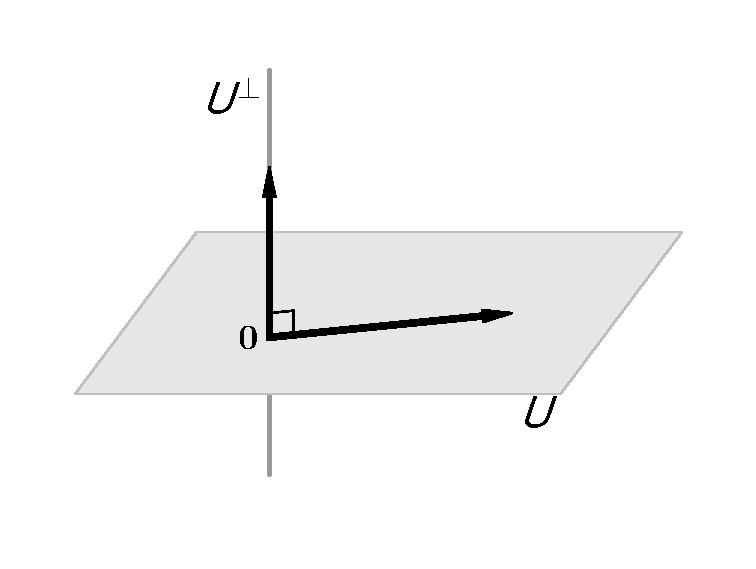
\includegraphics[width=0.4\textwidth]{img/_orthogonal_complement.pdf}
            \caption{Orthogonal complement of a subspace $U \subseteq \mathbb{R}^3$}
        \end{figure}
\end{description}



\section{Projections}
Projections are methods to map high-dimensional data into a lower-dimensional space 
while minimizing the compression loss.\\
\marginnote{Orthogonal projection}
Let $V$ be a vector space and $U \subseteq V$ a subspace of $V$.
A linear mapping $\pi: V \rightarrow U$ is a (orthogonal) projection if:
\[ \pi^2 = \pi \circ \pi = \pi \]
In other words, applying $\pi$ multiple times gives the same result (i.e. idempotency).\\
$\pi$ can be expressed as a transformation matrix $\matr{P}_\pi$ such that:
\[ \matr{P}_\pi^2 = \matr{P}_\pi \] 

\subsection{Projection onto general subspaces} \marginnote{Projection onto subspace basis}
To project a vector $\vec{x} \in \mathbb{R}^n$ into a lower-dimensional subspace $U \subseteq \mathbb{R}^n$,
it is possible to use the basis of $U$.\\
%
Let $m = \text{dim}(U)$ be the dimension of $U$ and 
$\matr{B} = (\vec{b}_1, \dots, \vec{b}_m) \in \mathbb{R}^{n \times m}$ an ordered basis of $U$.
A projection $\pi_U(\vec{x})$ represents $\vec{x}$ as a linear combination of the basis:
\[ \pi_U(\vec{x}) = \sum_{i=1}^{m} \lambda_i \vec{b}_i = \matr{B}\vec{\uplambda} \]
where $\vec{\uplambda} = (\lambda_1, \dots, \lambda_m)^T \in \mathbb{R}^{m}$ are the new coordinates of $\vec{x}$ 
and is found by minimizing the distance between $\pi_U(\vec{x})$ and $\vec{x}$.



\section{Eigenvectors and eigenvalues}

Given a square matrix $\matr{A} \in \mathbb{R}^{n \times n}$, 
$\lambda \in \mathbb{C}$ is an eigenvalue of $\matr{A}$ \marginnote{Eigenvalue}
with corresponding eigenvector $\vec{x} \in \mathbb{R}^n \smallsetminus \{ \nullvec \}$ if: \marginnote{Eigenvector}
\[ \matr{A}\vec{x} = \lambda\vec{x} \]

It is equivalent to say that:
\begin{itemize}
    \item $\lambda$ is an eigenvalue of $\matr{A} \in \mathbb{R}^{n \times n}$
    \item $\exists \vec{x} \in \mathbb{R}^n \smallsetminus \{ \nullvec \}$ s.t. $\matr{A}\vec{x} = \lambda\vec{x}$ \\
        Equivalently the system $(\matr{A} - \lambda \matr{I}_n)\vec{x} = \nullvec$ is non-trivial ($\vec{x} \neq \nullvec$).
    \item $\text{rank}(\matr{A} - \lambda \matr{I}_n) < n$
    \item $\det(\matr{A} - \lambda \matr{I}_n) = 0$ (i.e. $(\matr{A} - \lambda \matr{I}_n)$ is singular {\footnotesize(i.e. not invertible)})
\end{itemize}

Note that eigenvectors are not unique.
Given an eigenvector $\vec{x}$ of $\matr{A}$ with eigenvalue $\lambda$, 
we can prove that $\forall c \in \mathbb{R} \smallsetminus \{0\}:$ $c\vec{x}$ is an eigenvector of $\matr{A}$:
\[ \matr{A}(c\vec{x}) = c(\matr{A}\vec{x}) = c\lambda\vec{x} = \lambda(c\vec{x}) \]

% \begin{theorem}
%     The eigenvalues of a symmetric matrix $\matr{A} \in \mathbb{R}^{n \times n}$ are all in $\mathbb{R}$.
% \end{theorem}

\begin{theorem} \marginnote{Eigenvalues and positive definiteness}
    $\matr{A} \in \mathbb{R}^{n \times n}$ is symmetric positive definite $\iff$
    its eigenvalues are all positive.
\end{theorem}

\begin{description}
    \item[Eigenspace] \marginnote{Eigenspace}
        Set of all the eigenvectors of $\matr{A} \in \mathbb{R}^{n \times n}$ associated to an eigenvalue $\lambda$.
        This set is a subspace of $\mathbb{R}^n$.
    
    \item[Eigenspectrum] \marginnote{Eigenspectrum}
        Set of all eigenvalues of $\matr{A} \in \mathbb{R}^{n \times n}$.
\end{description}


\begin{description}
    \item[Geometric multiplicity] \marginnote{Geometric multiplicity}
        Given an eigenvalue $\lambda$ of a matrix $\matr{A} \in \mathbb{R}^{n \times n}$.
        The geometric multiplicity of $\lambda$ is the number of linearly independent eigenvectors associated to $\lambda$.
\end{description}


\begin{theorem} \marginnote{Linearly independent eigenvectors}
    Given a matrix $\matr{A} \in \mathbb{R}^{n \times n}$. 
    If its $n$ eigenvectors $\vec{x}_1, \dots, \vec{x}_n$ are associated to distinct eigenvalues, 
    then $\vec{x}_1, \dots, \vec{x}_n$ are linearly independent (i.e. they form a basis of $\mathbb{R}^n$).

    \begin{descriptionlist}
        \item[Defective matrix] \marginnote{Defective matrix}
            A matrix $\matr{A} \in \mathbb{R}^{n \times n}$ is defective if it has less than $n$ linearly independent eigenvectors.
    \end{descriptionlist}
\end{theorem}


\begin{theorem}[Spectral theorem] \label{th:spectral_theorem} \marginnote{Spectral theorem}
    Given a symmetric matrix $\matr{A} \in \mathbb{R}^{n \times n}$.
    Its eigenvectors form an orthonormal basis and its eigenvalues are all in $\mathbb{R}$.
\end{theorem}


\subsection{Diagonalizability}
\marginnote{Diagonalizable matrix}
A matrix $\matr{A} \in \mathbb{R}^{n \times n}$ is diagonalizable if it is similar to a diagonal matrix $\matr{D} \in \mathbb{R}^{n \times n}$:
\[ \exists \matr{P} \in \mathbb{R}^{n \times n} \text{ s.t. } \matr{P} \text{ invertible and } \matr{D} = \matr{P}^{-1}\matr{A}\matr{P} \]

\begin{theorem}
    Similar matrices have the same eigenvalues.
\end{theorem}

\begin{theorem} \marginnote{Symmetric matrix diagonalizability}
    A symmetric matrix $\matr{A} \in \mathbb{R}^{n \times n}$ is always diagonalizable.
\end{theorem}